\documentclass{../../oss-apphys-exam}
\usepackage{bm}
\usepackage{circuitikz} % to draw circuits!

\begin{document}
\genheader

\genfreetitle{C}{MAGNETISM}{5}

\genfreedirections
  
%TAKEN FROM 2002 AP PHYSICS C FREE-RESPONSE QUESTION E&M 3
\cpic{.55}{flux-through-loop}

\begin{questions}
  \question A circular wire loop with radius \SI{.10}{\metre} and resistance
  \SI{50}{\ohm} is suspended horizontally in a magnetic field of magnitude $B$
  directed upward at an angle of \ang{60} with the vertical, as shown above.
  The magnitude of the field in teslas is given as a function of time $t$ in
  seconds by the equation $B=4(1-0.2t)$.
  \begin{parts}
    \part Determine the magnetic flux $\Phi_m$ through the loop as a function of
    time.
    
    \part Graph the magnetic flux $\Phi_m$ as a function of time on the axes
    below.
    \begin{center}
      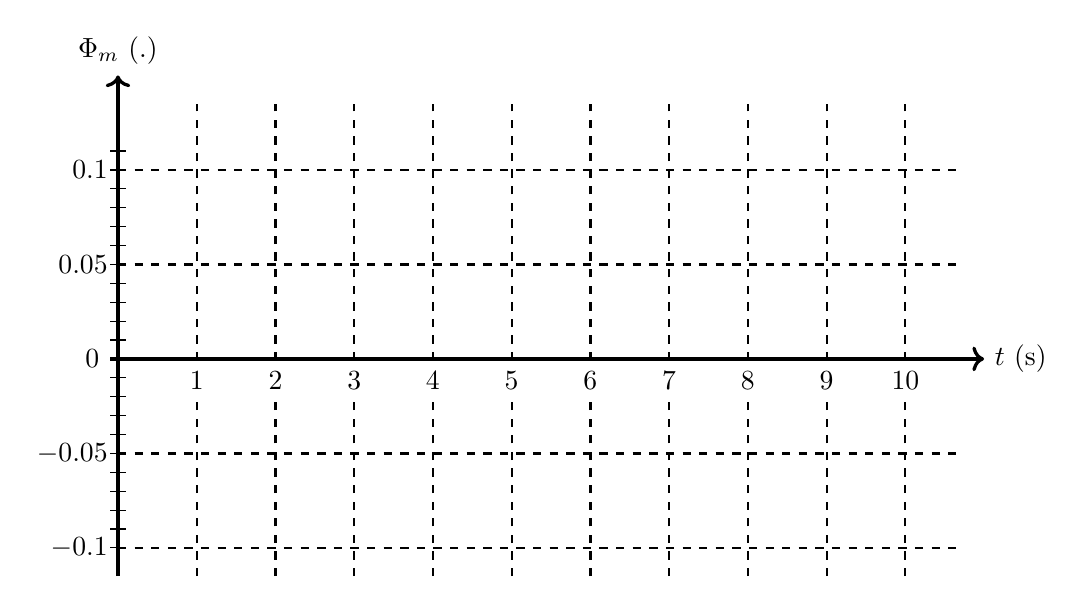
\begin{tikzpicture}[yscale=1.2]
        \draw[very thick,->](-.1,0)--(11,0) node[pos=0,left]{0}
        node[right]{$t$ (s)};
        \draw[very thick,->](0,-2.3)--(0,3)
        node[above]{$\Phi_m$ (\si{\tesla.\metre\squared})};
        \foreach\x in {1,...,10}{
          \draw[thick,dashed](\x,-2.3)--(\x,2.7);
          \node[fill=white,below] at (\x,-.03) {$\x$};
        }
        \foreach\y in {-0.1,-0.05,0.05,0.1}
        \draw[thick,dashed](0,\y*20)--(10.7,\y*20) node[pos=0,left]{$\y$};
        \foreach\y in {-2,-1.8,...,2.2} \draw(-.1,\y)--(.1,\y);
      \end{tikzpicture}
    \end{center}
    
    \part Determine the magnitude of the induced emf in the loop.

    \part
    \begin{subparts}
      \subpart Determine the magnitude of the induced current in the loop.
      \subpart Show the direction of the induced current on the following
      diagram.
    \end{subparts}
    \cpic{.55}{flux-through-loop}
  \end{parts}
  \newpage

  % TAKEN FROM 2004 AP PHYSICS C EXAM FREE-RESPONSE QUESTION E&M 3. THERE ARE
  % A LOT OF PROBLEMS THAT ARE VERY SIMILAR TO THIS ONE.
  \uplevel{
    \centering
    \begin{tikzpicture}
      \draw[thick](0,0) rectangle(4,3);
      \draw[|<->|](0,3.3)--(4,3.3) node[midway,fill=white]{$4\ell$};
      \draw[|<->|](-.4,0)--(-.4,3) node[midway,fill=white]{$3\ell$};
      \draw[|<->|](-.4,0)--(-.4,-1) node[midway,fill=white]{$\ell$};
      \draw[thick,->](-2,-1)--(2,-1) node[below]{$I$};
      \draw[thick](1.9,-1)--(6,-1);
    \end{tikzpicture}
  }
  \question A rectangular loop of dimensions $3\ell$ and $4\ell$ lies in the
  plane of the page as shown above. A long straight wire also in the plane of
  the page carries a current $I$.
  \begin{parts}
    \part Calculate the magnetic flux through the rectangular loop in terms of
    $I$, $\ell$, and fundamental constants.
    
    \uplevel{
      Starting at time $t=0$, the current in the long straight wire is given as
      a function of time $t$ by $I(t)=I_0e^{-kt}$, where $I_0$ and $k$ are
      constants.
    }

    \part The current induced in the loop is in which direction? Justify your
    answer.

    \vspace{.15in}
    \underline{\hspace{.5in}} Clockwise \hspace{1in}
    \underline{\hspace{.5in}} Counterclockwise

    \uplevel{
      The loop has a resistance $R$. Calculate each of the following in terms
      of $R$, $I_0$, $k$, $\ell$, and fundamental constants.
    }
    \part The current in the loop as a function of time $t$
    
    \part The total energy dissipated in the loop from $t=0$ to $t=\infty$
  \end{parts}
  \newpage

  \uplevel{
    \centering
    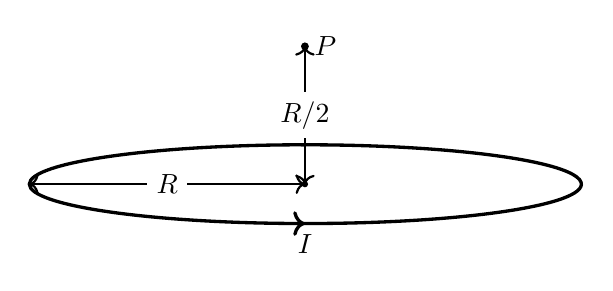
\begin{tikzpicture}[scale=.5]
      \draw[very thick,->](0,1)  arc(90:270:7 and 1) node[below]{$I$};
      \draw[very thick](-.1,-1) arc(-91:91:7 and 1);
      \fill(0,0) circle(.08);
      \draw[thick,<->](-7,0)--(0,0) node[midway,fill=white]{$R$};
      \draw[thick,<->](0,3.5)--(0,0) node[midway,fill=white]{$R/2$};
      \fill(0,3.5) circle(.1) node[right]{$P$};
    \end{tikzpicture}
    
    Figure 1
  }
  \question The circular loop of wire in Figure 1 above has a radius of $R$ and
  carries a current $I$. Point $P$ is a distance of $R_2$ above the center of
  the loop. Express algebraic answers to parts (a) and (b) in terms of $R$,
  $I$, and fundamental constants.
  \begin{parts}
    \part
    \begin{subparts}
      \subpart State the direction of the magnetic field $B_1$ at point $P$ due
      to the current in the loop.
      
      \subpart Calculate the magnitude of the magnetic field $B_1$ at point $P$.
    \end{subparts}

    \uplevel{
      \begin{center}
        \begin{minipage}{.45\textwidth}
          \centering
          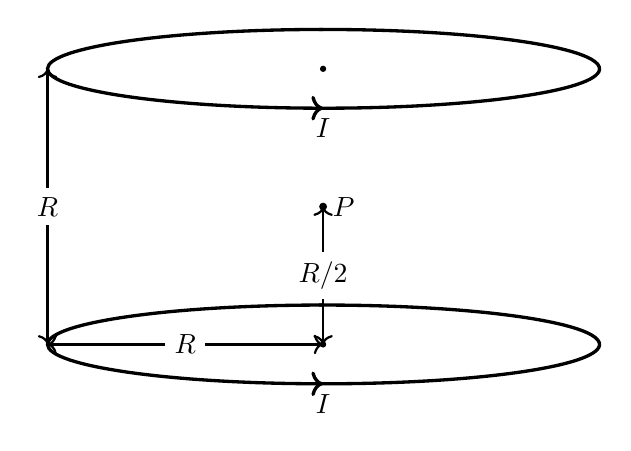
\begin{tikzpicture}[scale=.5]
            \draw[very thick,->](0,1)  arc(90:270:7 and 1) node[below]{$I$};
            \draw[very thick](-.1,-1) arc(-91:91:7 and 1);
            \fill(0,0) circle(.08);
            \draw[thick,<->](-7,0)--(0,0) node[midway,fill=white]{$R$};
            \draw[thick,<->](0,3.5)--(0,0) node[midway,fill=white]{$R/2$};
            \fill(0,3.5) circle(.1) node[right]{$P$};
            
            \draw[very thick,->](0,8)  arc(90:270:7 and 1) node[below]{$I$};
            \draw[very thick](-.1,6) arc(-91:91:7 and 1);
            \fill(0,7) circle(.08);
            
            \draw[thick,<->](-7,0)--(-7,7) node[midway,fill=white]{$R$};
          \end{tikzpicture}
        
          Figure 2
        \end{minipage}
        \begin{minipage}{.45\textwidth}
          \centering
          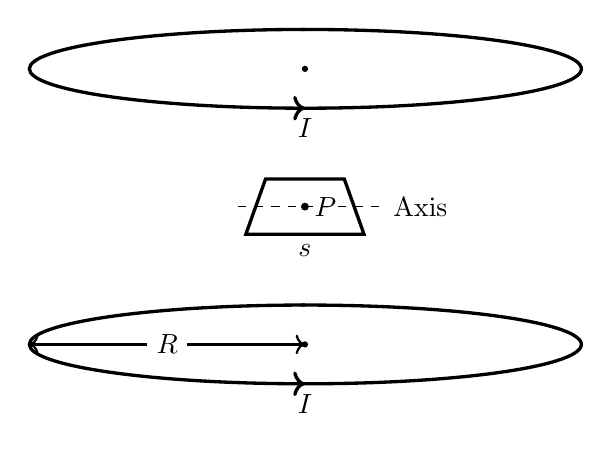
\begin{tikzpicture}[scale=.5]
            \draw[very thick,->](0,1)  arc(90:270:7 and 1) node[below]{$I$};
            \draw[very thick](-.1,-1) arc(-91:91:7 and 1);
            \fill(0,0) circle(.08);
            \draw[thick,<->](-7,0)--(0,0) node[midway,fill=white]{$R$};
            \fill(0,3.5) circle(.1) node[right]{$P$};
            
            \draw[very thick,->](0,8)  arc(90:270:7 and 1) node[below]{$I$};
            \draw[very thick](-.1,6) arc(-91:91:7 and 1);
            \fill(0,7) circle(.08);
            
            \draw[dashed](-1.7,3.5)--(2,3.5) node[right]{Axis};
            \draw[very thick](-1.5,2.8)--(1.5,2.8) node[midway,below]{$s$}
            --(1,4.2)--(-1,4.2)--cycle;
          \end{tikzpicture}

          Figure 3
        \end{minipage}
      \end{center}
      
      \vspace{.2in}A second identical loop also carrying a current $I$ is added
      at a distance of $R$ above the first loop, as shown in Figure 2 above.
    }

    \part Determine the magnitude of the net magnetic field $B$ net at point
    $P$.

    \uplevel{
      A small square loop of wire in which each side has a length $s$ is now
      placed at point $P$ with its plane parallel to the plane of each loop, as
      shown in Figure 3 above. For parts (c) and (d), assume that the magnetic
      field between the two circular loops is uniform in the region of the
      square loop and has magnitude $B_\text{net}$.
    }
    
    \part In terms of $B_\text{net}$ and $s$, determine the magnetic flux
    through the square loop.

    \part The square loop is now rotated about an axis in its plane at an
    angular speed $\omega$. In terms of $B_\text{net}$ , $s$, and $\omega$,
    calculate the induced emf in the loop as a function of time $t$, assuming
    that the loop is horizontal at $t=0$.
  \end{parts}
  \newpage
  
  \uplevel{
    \cpic{.5}{inout}
  }
  \question The rectangular loop of wire shown on the left in the figure above
  has mass $M$, length $L$, width $L/4$, and resistance $R$. It is initially
  moving to the right at constant speed $\varv_0$ , with no net force acting on
  it. At time $t=0$ the loop enters a region of length $2L$ that contains a
  uniform magnetic field of magnitude $B$ directed into the page. The loop
  emerges from the field at time $t_f$ with final speed $\varv_f$. Express all
  algebraic answers to the following in terms of $M$, $L$, $R$, $B$, $\varv_0$,
  and fundamental constants, as appropriate.
  \begin{parts}
    \part Let $x$ represent the position of the right end of the loop. Place a
    check mark in the appropriate box in each column in the table below to
    indicate whether the speed of the loop increases, decreases, or stays the
    same as the loop moves to the right.


    \part Derive an expression for the magnitude of the current induced in the
    loop as its right edge enters the field.

    \part What is the direction of the induced current determined in part (b) ?
    Justify your answer.

    \vspace{.15in}
    \underline{\hspace{.5in}} Clockwise\hspace{.6in}
    \underline{\hspace{.5in}} Counterclockwise
    
    \part Write, but do not solve, a differential equation for the speed
    $\varv$ as a function of time as the loop enters the field.
    
    \part What is the direction of the acceleration of the loop just before
    its left edge leaves the field? Justify your answer.

    \vspace{.15in}
    \underline{\hspace{.5in}} Left\hspace{1in}
    \underline{\hspace{.5in}} Right\hspace{1in}
    \underline{\hspace{.5in}} Up\hspace{1in}
    \underline{\hspace{.5in}} Down
  \end{parts}
  \newpage

  \uplevel{
    \centering
    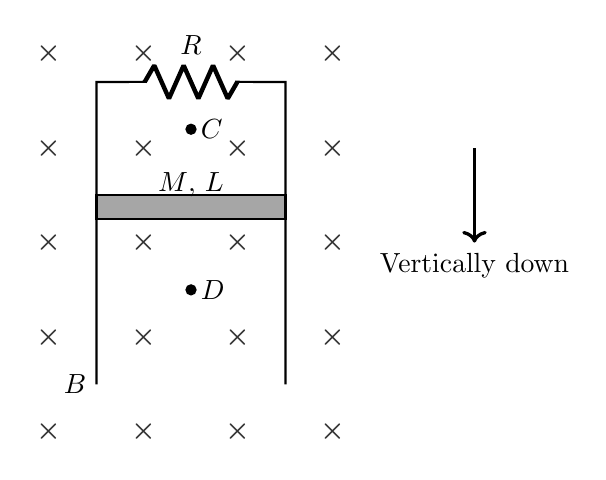
\begin{tikzpicture}[scale=1.2]
      \foreach \x in {0,...,3}{
        \foreach \y in {0,...,4}
        \node at (\x,\y){\textcolor{black!80}{$\bm\times$}};
      }
      \draw[thick,fill=gray!70](.5,2.25) rectangle(2.5,2.5)
      node[above,midway]{$M$, $L$};
      \draw[thick](.5,.5)--(.5,3.7) node[pos=0,left]{$B$}
      to[R,l=$R$](2.5,3.7)--(2.5,.5);
      \fill (1.5,1.5) circle(.06) node[right]{$D$};
      \fill (1.5,3.2) circle(.06) node[right]{$C$};
      \draw[very thick,->](4.5,3)--(4.5,2) node[below]{Vertically down};
    \end{tikzpicture}
  }
  \question A conducting bar of mass $M$, length $L$, and negligible resistance
  is connected to two long vertical conducting rails of negligible resistance.
  The two rails are connected by a resistor of resistance $R$ at the top. The
  entire apparatus is located in a magnetic field of magnitude $B$ directed
  into the page, as shown in the figure above. The bar is released from rest
  and slides without friction down the rails.
  \begin{parts}
    \part What is the direction of the current in the resistor?

    \vspace{.15in}
    \underline{\hspace{.5in}} Left\hspace{1in}
    \underline{\hspace{.5in}} Right

    \part
    \begin{subparts}
      \subpart Is the magnitude of the net magnetic field above the bar at
      point $C$ greater than, less than, or equal to the magnitude of the net
      magnetic field before the bar is released? Justify your answer.

      \vspace{.15in}
      \underline{\hspace{.5in}}Greater than\hspace{1in}
      \underline{\hspace{.5in}}Less than\hspace{1in}
      \underline{\hspace{.5in}}Equal to
      \vspace{.1in}
      
      \subpart While the bar is above point $D$, is the magnitude of the net
      magnetic field at point $D$ greater than, less than, or equal to the
      magnitude of the net magnetic field before the bar is released?
      Justify your answer.

      \vspace{.15in}
      \underline{\hspace{.5in}}Greater than\hspace{1in}
      \underline{\hspace{.5in}}Less than\hspace{1in}
      \underline{\hspace{.5in}}Equal to
      \vspace{.1in}
    \end{subparts}
    
    \uplevel{
      Express your answers to parts (c) and (d) in terms of $M$, $L$, $R$, $B$,
      and physical constants, as appropriate.
    }

    \part Write, but do NOT solve, a differential equation that could be used
    to determine the velocity of the falling bar as a function of time $t$.
    
    \part Determine an expression for the terminal velocity $v_T$ of the bar.

    \uplevel{
      Express your answers to parts (e) and (f) in terms of $v_T$, $M$, $L$,
      $R$, $B$, and physical constants, as appropriate.
    }
    
    \part Derive an expression for the power dissipated in the resistor when
    the bar is falling at terminal velocity.

    \part Using your differential equation from part (c), derive an expression
    for the speed of the falling bar $v_t$ as a function of time $t$.
  \end{parts}

  
%  % TAKEN FROM 2004 AP PHYSICS C EXAM FREE-RESPONSE QUESTION E&M 2.
%  % THIS QUESTION IS BETTER SUITED FOR THE ELECTRIC CIRCUIT SECTION, BUT IS
%  % HERE FOR SOME REASON. I MIGHT MOVE IT TO HW 16 LATER.
%  
%  \cpic{.85}{RC2004}
%  \question In the circuit shown above left, the switch $S$ is initially in the
%  open position and the capacitor $C$ is initially uncharged. A voltage probe
%  and a computer (not shown) are used to measure the potential difference
%  across the capacitor as a function of time after the switch is closed. The
%  graph produced by the computer is shown above right. The battery has an emf
%  of \SI{20}{\volt} and negligible internal resistance. Resistor $R_1$ has a
%  resistance of \SI{15}{\kilo\ohm} and the capacitor $C$ has a capacitance of
%  \SI{20}{\micro\farad}.
%  \begin{parts}
%    \part Determine the voltage across resistor $R_2$ immediately after the
%    switch is closed.
%    
%    \part Determine the voltage across resistor $R_2$ a long time after the
%    switch is closed.
%    
%    \part Calculate the value of the resistor $R_2$.
%    
%    \part Calculate the energy stored in the capacitor a long time after the
%    switch is closed.
%    
%    \part On the axes below, graph the current in $R_2$ as a function of time
%    from 0 to \SI{15}{\second}. Label the vertical axis with appropriate
%    values.
%    \begin{center}
%      \begin{tikzpicture}[xscale=.6,yscale=.35]
%        \draw[dashed](0,0) grid(15,20);
%        \draw[step=5,very thick](0,0) grid(15,20);
%        \foreach \x in {0,5,...,15} \node[below] at (\x,0) {$\x$};
%        \node[below] at (7.5,-1.5) {Time (s)};
%        \node[left] at (0,10) {Current in $R_2$};
%      \end{tikzpicture}
%    \end{center}
%    \uplevel{
%      Resistor $R_2$ is removed and replaced with another resistor of lesser
%      resistance. Switch $S$ remains closed for a long time.
%    }
%
%    \part Indicate below whether the energy stored in the capacitor is greater
%    than, less than, or the same as it was with resistor $R_2$ in the circuit.
%    Explain your reasoning.
%    
%    \vspace{.1in}
%    \underline{\hspace{.2in}} Greater than\hspace{.3in}
%    \underline{\hspace{.2in}} Less than\hspace{.3in}
%    \underline{\hspace{.2in}} The same as
%  \end{parts}
%  \newpage

  
%\item Two positive charges $+q$ are on the $y$ axis at $y=+a$ and $y=-a$.
%  \begin{enumerate}
%  \item Show that the electric field on the $x$ axis is along the $x$ axis with
%    $E_x=2kqx(x^2+a^2)^{-3/2}$.
%  \item Show that near the origin, when $x\ll a$, $E_x\approx 2kqx/a^3$.
%  \item Show that for $x\gg a$, $E_x\approx 2kq/x^2$.
%  \item Explain why you should expect the result in (c) even before calculating
%    it.
%  \end{enumerate}
%  A bead of mass $m$ with a negative charge $-q$ slides along a thread that
%  runs along the $x$ axis.
%  \begin{enumerate}[resume]
%  \item Show that for small displacements $x\ll a$, the bead experiences a
%    restoring force that is proportional to $x$ and therefore undergoes
%    simple harmonic motion.
%  \item Find the period of the motion.
%  \end{enumerate}
%  %\vspace{\stretch{4}}
%  \newpage
%  
%\item Using Gauss's law, find
%  \begin{enumerate}
%  \item the electric field strength inside and outside of a uniformly charged
%    hollow sphere of radius $R$ and surface charge density $\sigma$ (charge
%    per unit area).
%  \item the electric field inside and outside an infinitely long cyclindrical
%    shell of charge of radius $R$ with charge discibution $\sigma$ (charge
%    per unit area).
%  \item the electric field strength inside and outside a infinitely long solid
%    cylinder of radius $R$ carrying a linear uniform charge density $\rho$
%    (charge per unit volume).
%  \end{enumerate}
%  Hint: In all cases, think about where to put the Gaussian surface. Take
%  advantage of symmetry.
%  %\vspace{\stretch{1}}
%  \newpage

%\item A parallel-plate capacitor has a capacitance $C_0$ and plate separation
%  of $d$. To dielectric slabs of constants $\kappa_1$ and $\kappa_2$, each of
%  thickness $d/2$ and having the same area as the plates, are inserted between
%  the plates as shown in the figure below. When the free charge on the plates
%  are $Q$,
%  \begin{enumerate}
%  \item find the electric field in each of the dielectric
%  \item find the potential difference between the plates
%  \item show that the new capacitance is given by:
%    $C=\dfrac{\kappa_1\kappa_2}{\kappa_1+\kappa_2}C_0$
%  \end{enumerate}
%  \cpic{.2}{stacked}
\end{questions}
\end{document}
